\documentclass[%
paper=a4,						% alle weiteren Papierformat einstellbar
%landscape,						% Querformat
fontsize=11pt,					% Schriftgröße (12pt, 11pt (Standard))
%BCOR1cm,						% Bindekorrektur, bspw. 1 cm
DIV=calc,						% führt die Satzspiegelberechnung neu aus
								% s. scrguide 2.4
%twoside,						% Doppelseiten
%twocolumn,						% zweispaltiger Satz
parskip=half,					% Absatzformatierung s. scrguide 3.1
%headsepline,					% Trennline zum Seitenkopf	
%footsepline,					% Trennline zum Seitenfuß
titlepage,						% Titelei auf eigener Seite
headings=big,				% Überschriften etwas kleiner (smallheadings)
%idxtotoc,						% Index im Inhaltsverzeichnis
%liststotoc,					% Abb.- und Tab.verzeichnis im Inhalt
bibliography=totoc,				% Literaturverzeichnis im Inhalt
%abstracton,					% Überschrift über der Zusammenfassungan	
%leqno,   						% Nummerierung von Gleichungen links
%fleqn,							% Ausgabe von Gleichungen linksbündig
%draft							% überlangen Zeilen in Ausgabe gekennzeichnet
]
{scrartcl}

\usepackage[pdftex]{graphicx} 
\usepackage[ngerman]{babel}	
\usepackage[utf8]{inputenc}		
\usepackage[T1]{fontenc}								
\usepackage{lmodern}
\usepackage{color}
\usepackage{booktabs}
\usepackage{array}

% Links im PDF
\usepackage{hyperref}
\definecolor{LinkColor}{rgb}{0,0,0.5}
\hypersetup{
	colorlinks=true,
	linkcolor=LinkColor,
	citecolor=LinkColor,
	filecolor=LinkColor,
	menucolor=LinkColor,
	urlcolor=LinkColor}
	
%Kopf u. Fußzeilen
\usepackage{scrpage2}
\pagestyle{scrheadings}
\clearscrheadfoot
%\chead{}
%\ofoot{}
\cfoot{\pagemark}

\usepackage{mdwlist}
\usepackage{csquotes}

% Neues bibliographie paket
% style=apa
\usepackage[isbn=false,url=false, doi=false, backend=biber, style=numeric]{biblatex}
%\DeclareLanguageMapping{american}{american-apa}

\usepackage{pdfpages}

\def \varpressetext {<Pressetext angeben>}
\newcommand{\pressetext}[1]{\def \varpressetext {#1}}

\def \vargruppe {<Gruppennummer angeben>}
\newcommand{\gruppe}[1]{\def \vargruppe {#1}}

\def \varmitglieder {<Gruppenmitglieder angeben>}
\newcommand{\mitglieder}[1]{\def \varmitglieder {#1}}

\KOMAoptions{DIV=last}


\begin{document} 

\begin{titlepage}
\sffamily

{ \Large Forschungsmethoden WS 2012} \\[2cm]
    
{ \Huge \centering \bfseries Übung 4: Gesamt-Studienzusammenfassung \\[1.5cm] }

%{ \LARGE \centering \bfseries \varpressetext \\[1.5cm] }

%{
%    \begin{flushright}
%    { \large
%       { \bfseries Bewertete Gruppe:~\vargruppe \\ }
%       \varmitglieder
%    }
%
%    \end{flushright}
%}

\vfill

{ \large
   { \bfseries Gruppe: 8 \\ }
   Bernhard Fleck \\
   Rafael Konik \\
   Stephan Matiasch \\
   Harald Watzke \\
}
\end{titlepage}


\section{Gesamtzusammenfassung aller Studien} % (fold)
\label{sec:zusammenfassung_aller_studien}

\begin{figure}[h!tbp]
    \begin{center}
        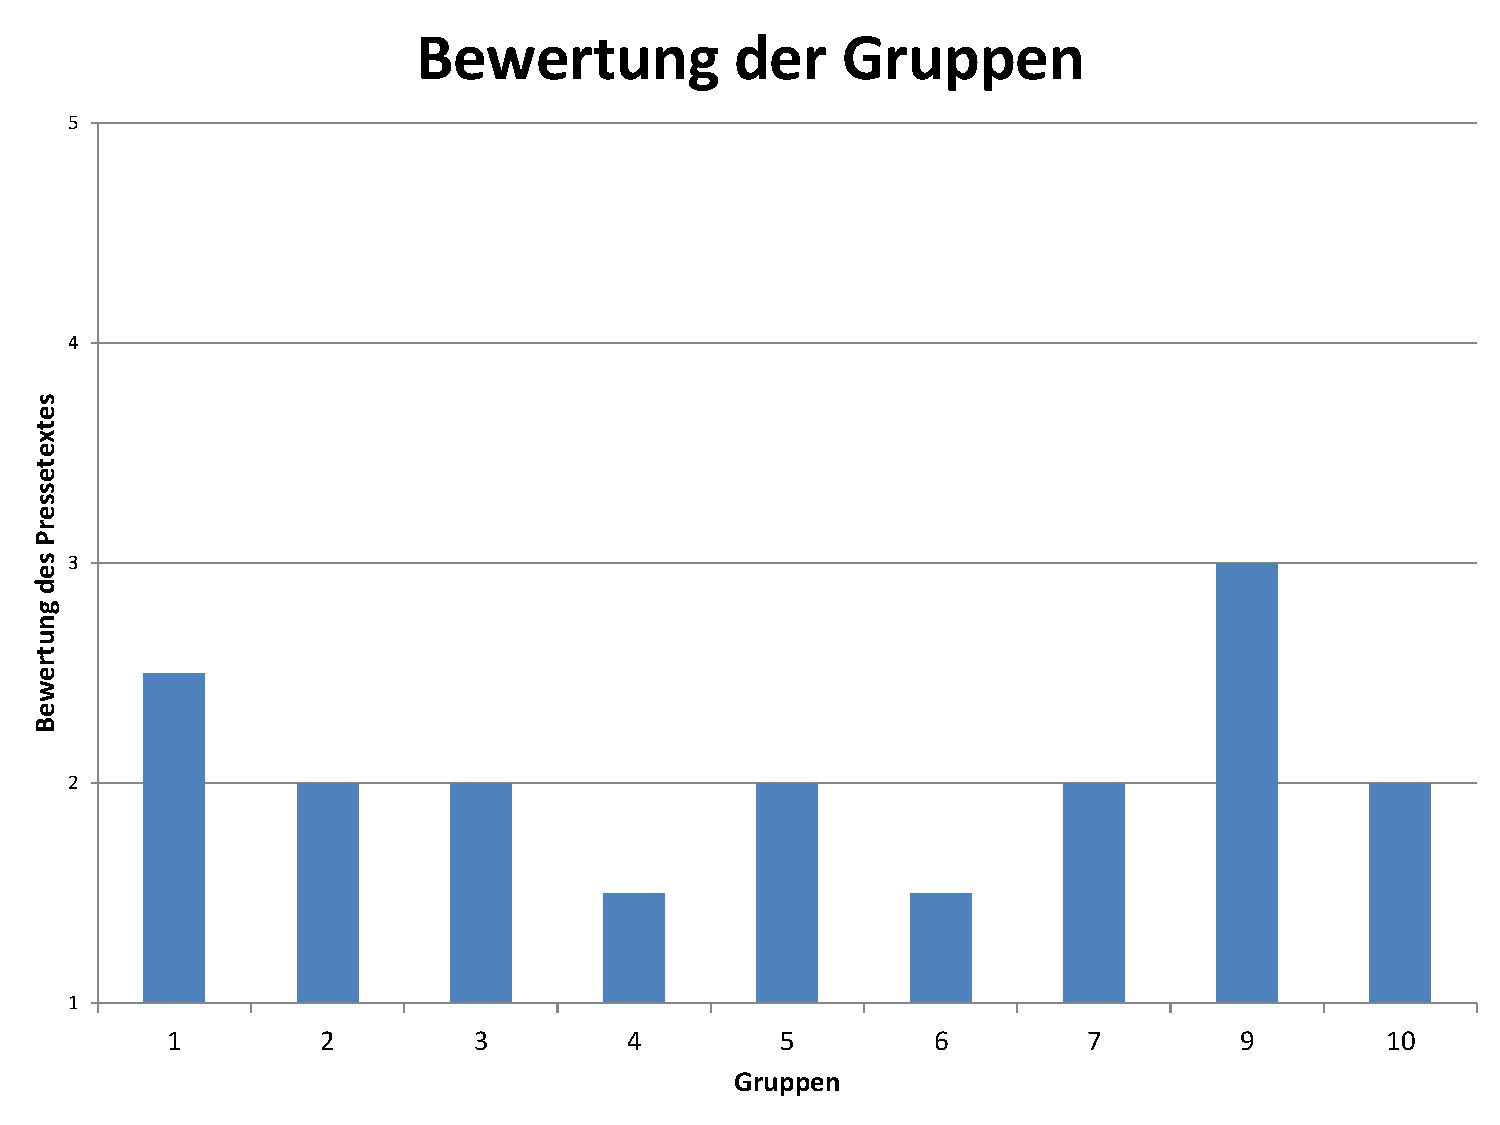
\includegraphics[width=\textwidth]{images/bewertungen}
    \end{center}
    \caption{Bewertung der Pressetexte. Die Zahlen 
    stehen von 1 bis 5 für: \enquote{gut gefallen}, \enquote{eher gut 
    gefallen}, \enquote{weder noch}, \enquote{eher nicht gefallen} und 
    \enquote{nicht gefallen}}
    \label{fig:bewertungen}
\end{figure}

\begin{figure}[h!tbp]
    \begin{center}
        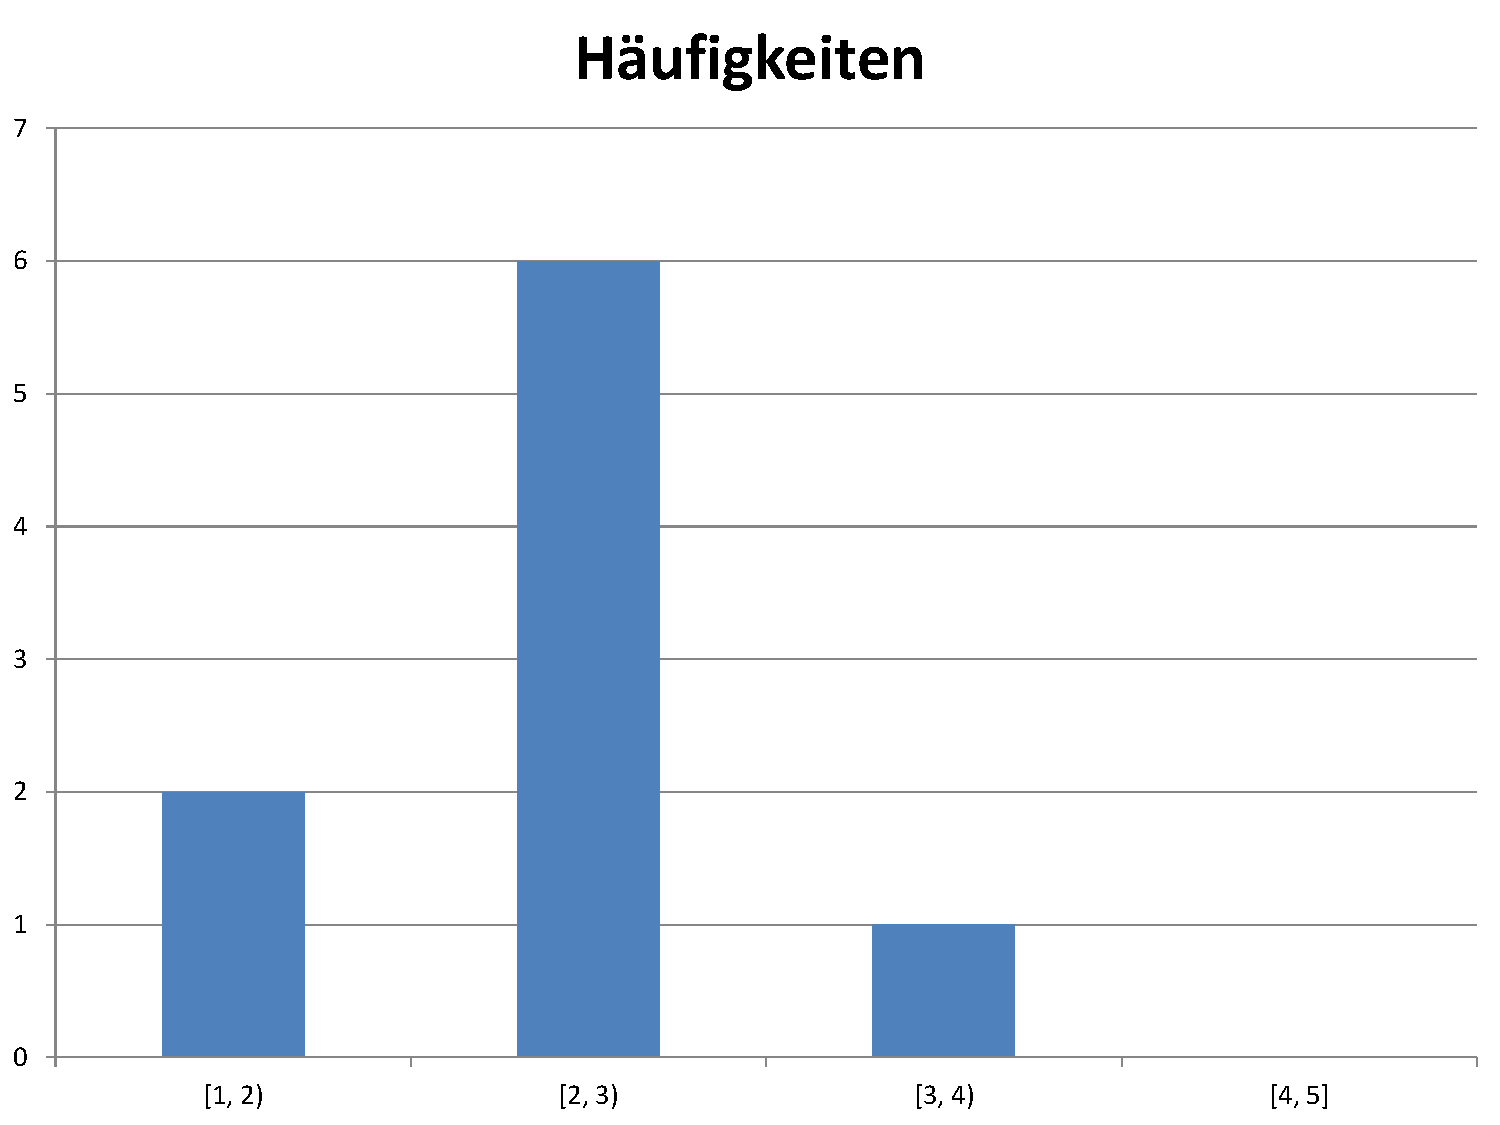
\includegraphics[width=\textwidth]{images/haeufigkeiten}
    \end{center}
    \caption{Häufigkeiten der Bewertungen. Die Zahlen 
    stehen von 1 bis 5 für: \enquote{gut gefallen}, \enquote{eher gut 
    gefallen}, \enquote{weder noch}, \enquote{eher nicht gefallen} und 
    \enquote{nicht gefallen}}
    \label{fig:haeufigkeiten}
\end{figure}

% section zusammenfassung_aller_studien (end)

\end{document}